\chapter{Dynamic development of nanometer scale grain boundaries during liquid phase sintering}

\section{Introduction}

During sintering of ceramics insoluble impurities and dopants can accumulate in the grain boundaries and form an amorphous grain boundary film that significantly influences the sintering behavior and properties of ceramics. Recently, it has been established that grain boundaries in fully dense microstructures can possess different characteristics, depending on chemistry and temperature. Based on their structure and thickness, grain boundaries have been classified into different types of thermodynamically stable complexions \cite{Dillon2007}. The type of complexion strongly affects transport kinetics and determines the mobility of a grain boundary, and if multiple complexions coexist at a time, multi-modal grain-size distributions and anisotropic microstructures can develop. One class of grain boundaries that is well investigated in dense ceramics are intergranular films (IGF), since they are often observed in a variety of systems such as Si$_{3}$N$_{4}$, SiC, and Al$_{2}$O$_{3}$ \cite{Subramaniam2006,Clarke1993}. IGFs are amorphous grain boundary films with an equilibrium thickness of typically 1-2 nm. Clarke et al. showed that the equilibrium film thickness results from a balance of attractive and repulsive interparticle forces, similar to those seen in colloidal systems \cite{Clarke1987,Clarke1993}.

In classical sintering theories the differences in grain boundary structures are considered by distinguishing between solid state and liquid phase sintering with fundamental differences in their respective sintering mechanisms. Solid state sintering occurs by solid state diffusion throughout the entire sintering process. During initial stage sintering surface diffusion leads to the formation of necks between particles. Most of the densification up to $\sim$92\% occurs during intermediate stage, where grain boundaries between particles and pore channels along the grain edges form. At densities >92\% the pore channels close and isolated pores first form and are then eliminated during final stage sintering. The dominant diffusion mechanisms during intermediate and final stage sintering are volume and grain boundary diffusion, which can be affected by solute segregated to the grain boundaries \cite{Dillon2007}. 

In contrast, for liquid phase sintering \cite{Kingery2004} the particle compact is penetrated by a liquid film and during the initial sintering stage the powder compact begins to densify by particle rearrangement after the liquid phase has formed. Further densification during intermediate and final stage sintering is controlled by a solution-precipitation mechanism, where the particles of the sinter are dispersed in a liquid glass matrix, and material from the grain boundary area dissolves into the liquid grain boundary phase and diffuses to the particle necks, where it precipitates, leading to a particle contact flattening and densification.

Additional models were developed in the literature that account for the liquid phase redistribution during densification. For example, a number of models describe the filling of pores during liquid phase sintering due to capillarity \cite{Lee1998,Shaw1986}. However, the existing models in the literature that address liquid phase redistribution typically deal with liquid concentrations of at least a few volume percent. In this case it can be assumed that the concentration of liquid phase is high enough to form a continuous liquid film of equilibrium thickness \cite{Subramaniam2006,Clarke1987,Clarke1993} in the grain boundaries and that excess liquid phase accumulates in necks, pores and glass pockets. For example, Svoboda et al.\cite{Svoboda1996} assumed a constant equilibrium intergranular film thickness of 1.5 nm when they developed their liquid phase sintering model, and Kwon and Messing \cite{Kwon1991} estimated a grain boundary thickness of $\sim$1 nm based on a squeeze film analysis. 

The redistribution of liquid phase becomes more complicated as the liquid phase concentration in a sinter is reduced, for example to concentrations <0.2 vol.\%. In this case the glass phase concentration could be insufficient to form a liquid film of equilibrium thickness, and if the glass phase concentration is low enough the grain boundaries may be considered rather solid than liquid, which changes the sintering model that can be applied. This case is interesting specifically in commercial powders used in industry, since they typically contain higher impurity levels than the ultrahigh purity powders studied in academia. For example, most fundamental research on alumina uses ultrahigh purity aluminas of >99.99\% Al$_{2}$O$_{3}$ and, therefore, sintering is analyzed using solid state sintering models. In contrast commercial alumina powders are typically produced by the Bayer process and are $\sim$99.8\% pure with ppm levels of Na$_{2}$O, SiO$_{2}$, CaO, and Fe$_{2}$O$_{3}$, and added MgO as a sintering additive. The concentration and ratios of these impurities and additives can vary substantially by the commercial grade and can form a small amount of liquid phase. Despite considerable interest no research has been done on determining what volume fraction of liquid phase is necessary to consider grain boundaries liquid and when to apply a liquid phase sintering model in such a system. 

Concentration, chemistry, and distribution of a liquid phase change during densification as a result of increasing temperature during heating and as a result of changing grain boundary area during densification and grain growth. This implies that grain boundaries undergo a dynamic change in physical and chemical character during densification. This dynamic change in chemistry and structure and possible transitions of grain boundaries from solid to liquid or vice versa can significantly impact densification as densification typically occurs via grain boundary diffusion. While most liquid phase sintering models imply that grain boundaries may change during densification, no work has been done on identifying these changes.

In this work we develop a physical model to predict the dynamic development of grain boundaries from initial to final stage sintering as a function of chemical and physical parameters of a sintering powder. The predicted grain boundary thicknesses are compared with grain boundaries examined by high-resolution TEM. 

\section{Experiment}

Two chemically purified Bayer process alumina powders (Almatis, Inc., Leetsdale, PA, USA) were chosen for this study. Powder characteristics and experimental details are described in previous chapter. The main difference between the two powders are the MgO concentrations of 2 ppm (MgO-free powder) and 380 ppm (MgO-doped powder), respectively. The powders were doped with up to 1000 ppm Na$_{2}$O and 1000 ppm SiO$_{2}$ using sodium acetate (NaC$_{2}$H$_{3}$O$_{2}$$\cdot$3H$_{2}$O, ACS grade, BDH, VWR International LLC, West Chester, PA, USA) and tetraethyl orthosilicate (Si(OC$_{2}$H$_{5}$)$_{4}$, 98\%, Aldrich Chemical Company, Inc. Milwaukee, WI, USA), respectively, to obtain chemistries similar to commercial high purity Bayer aluminas at different glass concentrations. Samples with green densities of 59.0 $\pm$ 0.5\% were fabricated for sintering studies by uniaxial and cold isostatic dry pressing (CIP, Autoclave engineers, Erie, Pa, USA) at 170 MPa and 200 MPa, respectively. The dry pressed cylinders were heated at 10$^{\circ}$C/min to 1525$^{\circ}$C in a thermomechanical analyzer (TMA, Linseis PT1600, Robbinsville, NJ, USA) to record the shrinkage during heating. Samples were heated at 10$^{\circ}$C/min to 1200$^{\circ}$C and then at 5$^{\circ}$C/min to 1525$^{\circ}$C for different hold times. Microstructure and density were measured by the linear intercept (ASTM Standard E112-96) \cite{Standard2013} and Archimedes methods (ASTM standard B962-15), \cite{Standard2015} respectively. The structure and chemistry of grain boundaries were investigated by transmission electron microscopy (TEM) and energy dispersive x-ray spectroscopy (EDS) using a dual aberration corrected FEI Titan \cite{Clarke1987} field emission microscope operated at 300 kV and FEI Talos (FEI, Hillsboro, OR, USA) field emission microscope at 200 kV. The EDS on both microscopes is an FEI Super-X system consisting of four SDDs (Silicon Drift Detectors) with a solid angle of 0.9 srad. The samples for TEM and EDS were air-quenched from the sintering temperature and prepared using a focused ion beam (Quanta 200 3D Dual Beam FIB, FEI, Hillsboro, OR, USA).  Grain boundaries were chosen for analysis that were oriented parallel to the TEM beam in order to accurately measure grain boundary thicknesses in the 2D projection images and EDS profiles.

\section{Grain boundary thickness in MgO-free alumina}
The development of the grain boundary thickness during densification is described for MgO-free powder samples with 529/103 ppm Na$_{2}$O/SiO$_{2}$, 529/203 ppm Na$_{2}$O/SiO$_{2}$, and 529/603 ppm Na$_{2}$O/SiO$_{2}$. As shown in the previous chapter, the main difference of the samples is the concentration of glass phase that forms. The liquidus projection of the Al$_{2}$O$_{3}$-Na$_{2}$O-SiO$_{2}$ phase diagram \cite{Svoboda1996} was used to predict the equilibrium composition of the glass phase during heating as a function of temperature \cite{Frueh2016a}, and based on the concentration of Na$_{2}$O and SiO$_{2}$ the glass phase concentration $\phi(T)$ was estimated as a function of temperature, as shown in Figure \ref{Ch4-figure:Figure1}. 

The liquid glass is expected to accumulate in particle contacts due to capillary forces \cite{Shaw1986}, and during densification it is assumed that the liquid phase accumulates in the grain boundaries until an equilibrium film thickness \cite{Subramaniam2006} is reached. After this equilibrium thickness is reached it is assumed that the excess liquid phase accumulates in the particle necks. The fraction of a particle/grain surface that is in contact with another particle/grain, i.e. the fraction of grain boundary area, increases with increasing density \cite{German2016}:

%%
\begin{equation}
\label{Ch4-eq: eq1}
\alpha(\rho) = 1 - r(\rho) \left(1-\frac{\rho}{100} \right)^{\frac{1}{2}}
\end{equation}
%%

\noindent where $r$ is a factor between 1.4 and 1.7, depending on the relative density. With these assumptions the grain boundary thickness based on the amount of impurities in the samples can be estimated by:

%%
\begin{equation}
\label{Ch4-eq: eq2}
\delta = 2 \frac{V_{g}\phi (T)}{S_{g}\left(1-\phi(T)\right)\alpha(\rho)}
\end{equation}
%%

\noindent where $V_{g}$ and $S_{g}$ are the average volume and average surface area of a particle/grain. The parameters of this equation are specific to the system investigated and change during sintering.

If the calculated grain boundary thickness is smaller than a monolayer, e.g. the size of a SiO$_{4}^{4-}$ tetrahedron ($\sim$0.3 nm) \cite{Clarke1987}, the liquid phase concentration in the sample is not high enough to form a liquid grain boundary phase, assuming a homogeneous distribution of the liquid phase in the sample. We assume that a grain boundary thickness > 0.6 nm, i.e. a bilayer of SiO$_{4}^{4-}$ tetrahedra, is necessary to consider the grain boundary liquid or liquid like. For calculated grain boundary thicknesses > 0.6 nm the grain boundary thickness is assumed to be limited by an equilibrium film thickness, if the concentration of the liquid phase is high enough to form an amorphous film of equilibrium thickness. If the concentration of the liquid phase is not high enough to form an amorphous film of equilibrium thickness, the grain boundary thickness is limited by the concentration of glass phase in the sample.

Dilatometry was used to determine the development of relative density as a function of temperature (Figure \ref{Ch4-figure:Figure2}), assuming isotropic shrinkage of the samples. Now the increase in liquid phase concentration can be expressed as a function of relative density, as seen in Figure \ref{Ch4-figure:Figure3}. $V_{g}$ and $S_{g}$ were estimated using the average particle/grain size determined from micrographs, assuming spherical particles of the same size. Using the sintering trajectories shown in Figure \ref{Ch4-figure:Figure4}, $V_{g}$ and $S_{g}$ can be expressed as a function of relative density. The grain boundary thickness can be calculated as a function of relative density since all parameters in Eq. \ref{Ch4-eq: eq2} can be expressed as a function of the relative density.

\section{The equilibrium film thickness model}
In 1987 Clarke proposed a model to calculate the equilibrium grain boundary thickness based on the equilibrium between attractive van der Waals and capillary pressures ($P_{vdW}$ and $P_{C}$) and a repulsive structural disjoining pressure ($P_{ST}$) \cite{Clarke1987}:

%%
\begin{equation}
\label{Ch4-eq: eq3}
P_{vdW} + P_{C} = P_{ST} 
\end{equation}
%%

\noindent The van der Waals pressure is given by

%%
\begin{equation}
\label{Ch4-eq: eq4}
P_{vdW} = \frac{A}{6 \pi h^{3}}
\end{equation}
%%

\noindent where $h$ is the grain boundary thickness and $A$ is the Hamaker constant, which can be estimated by:

%%
\begin{equation}
\label{Ch4-eq: eq5}
A = \frac{3}{4}kT\left( \frac{\varepsilon_{\alpha} - \varepsilon_{\beta}}{\varepsilon_{\alpha} + \varepsilon_{\beta}} \right)^{2} + \frac{3 \pi \hbar v}{8 \sqrt{2}} \frac{\left( n_{\alpha}^{2} - n_{\beta}^{2} \right)^{2}}{\left( n_{\alpha}^{2} + n_{\beta}^{2} \right)^{\frac{3}{2}}}
\end{equation}
%%

\noindent where $k$ is the Boltzmann constant, $T$ is the absolute temperature, $\varepsilon_{\alpha}$ and $\varepsilon_{\beta}$ are the dielectric constants of the ceramic and the glass phase, respectively, and $n_{\alpha}$ and $n_{\beta}$ are the refractive indices of the ceramic and the glass phase, respectively.

In Clarke's original work the capillary pressure was assumed to be constant, which is a valid assumption for samples at constant densities. However, during densification the capillary pressure changes and can be estimated by \cite{Kwon1991}:

%%
\begin{equation}
\label{Ch4-eq: eq6}
P_{C} = \frac{\left( 0.59-0.79 \left(1-\rho \right)^{\frac{1}{2}} \right) \rho^{\frac{1}{3}}}{0.39 \left(1-\rho \right)^{\frac{1}{2}} \left(0.59-0.39 \left(1-\rho \right)^{\frac{1}{2}} \right)} \frac{\gamma_{lv}}{r_{s}}
\end{equation}
%%

\noindent where $\gamma_{lv}$ is the surface tension of the liquid, $r_{s}$ is the particle radius, and $\rho$ is the relative sintered density.

The structural disjoining pressure is given by \cite{Clarke1987}:

%%
\begin{equation}
\label{Ch4-eq: eq7}
P_{ST} = - \alpha \tau_{0}^{2} \left( sinh^{2} \left( \frac{h}{2 \xi} \right) \right)^{-1}
\end{equation}
%%

\noindent where $a$ is a constant that can be approximated by the heat of fusion, $\tau_{0}$ is a coefficient for the degree of ordering between 0 and 1, and $\xi$ is a structural correlation length.

In later work Clarke et al. proposed that entropic repulsion of electrical double layers (EDL) could contribute to the pressure balance to stabilize intergranular films of equilibrium thickness, and used standard DLVO theory to describe the electric repulsive pressure \cite{Clarke1993}. EDLs are well studied in the literature \cite{Israelachvili2011} and consist of a first internal layer of adsorbed ions on the particle surface, i.e. the Stern layer, and a second, diffuse layer of counter ions that typically extents several nanometers of the diffuse layers of particles in suspension; however, it has been shown that if the separation distance of the particles and the structural size of the segregated species that form the Stern layer are in the same size range (e.g. at separation distances $\leq$ 2 nm) EDL interactions are negligible \cite{Israelachvili2011,Claesson1984}. Therefore, we believe that EDL interactions do not significantly contribute to the equilibrium thickness of interagranular films, since intergranular films are typically 1 - 2 nm thick. It is more likely that Stern layer interactions contribute to the separation distance rather than EDL contributions, if such layers form within the intergranular film around the alumina particles. Using molecular dynamics simulaitons Litton and Garofalini \cite{Zhang2005,Litton1999,Litton2000} showed that in siliceous intergranular films cations such as Na$^{+}$ and Ca$^{2+}$ can segregate to the surface of alumina particles. However, as discussed by Litton and Garofalini, the segregated ions serve as charge compensation rather than creating a charged Stern layer. Therefore, it is questionable if an EDL forms in the present system. 

For the purpose of this work we assume that no electric repulsive pressure contributes to the pressure balance and that the structural disjoining pressure is the only significant pressure, as originally proposed by Clarke et al. \cite{Clarke1993}. 

\section{Calculation of the theoretical Equilibrium Film Thicknesses}
To calculate the equilibrium film thickness for alumina samples, the contributions $P_{vdW}$, $P_{C}$, and $P_{ST}$ were calculated using parameters from the literature. The van der Waals pressure was estimated using Eq. \ref{Ch4-eq: eq3} and \ref{Ch4-eq: eq4} for a liquid sodium aluminosilicate glass film ($\varepsilon_{\beta}$ = 10 \cite{Hsieh1996}, $n_{\beta}$ = 1.51 \cite{Day1962}) located between two flat alumina surfaces ($\varepsilon_{\alpha}$ = 11.6, $n_{\alpha}$ = 1.752) \cite{Clarke1987}. The capillary pressure was calculated as a function of the relative density and grain size from the sintering trajectories shown in Figure \ref{Ch4-figure:Figure2}, using Eq. \ref{Ch4-eq: eq6}, assuming a surface tension of the sodium aluminosilicate glass of $\gamma_{glass}$ = 387 N/m \cite{Lyon1942}. The structural disjoining pressure was calculated using the heat of fusion of carnegieite (35.8 J/cm$^{3}$) for the constant $a$, and a structural correlation length of 0.3 nm (approximate size of a SiO$_{4}^{4-}$ tetrahedron). The heat of fusion of carnegieite was chosen since its chemical composition is close to the chemical composition of the grain boundary phase investigated here. It is reported in the literature that considerable ordering of intergranular fims can extend up to 1.5 nm into the intergranular film before they can be assumed completely amorphous \cite{Zhang2005}. Therefore, a high ordering factor of 0.75 was assumed.

Figure \ref{Ch4-figure:Figure5} shows the individual contributions to the equilibrium film thickness plotted as a function of film thickness for a sample with 529 ppm Na$_{2}$O and 603 ppm SiO$_{2}$ at 1525$^{\circ}$C and a relative density of 93\%. It can be seen that the net pressure, i.e. the sum of the acting pressures, is 0 MPa for a film thickness of 1.7 nm, which corresponds to the equilibrium film thickness. From the above discussion it is apparent that $P_{vdW}$ and $P_{CP}$ change during densification. The film thickness at which the net pressure is 0 MPa (i.e., the equilibrium film thickness) was calculated for samples at different relative densities during the sintering process, and the calculated equilibrium film thicknesses are shown in Figure \ref{Ch4-figure:Figure6}. It should be noted that $P_{vdW}$ and $P_{C}$ are a function of temperature, since the parameters they are calculated from are functions of temperature, glass composition, refractive indices, dielectric constants, and surface tension. However, investigations showed that the changes in $P_{vdW}$ and $P_{C}$ due to the changing temperature are insignificant, and therefore, these contributions were assumed to be constant. Figure \ref{Ch4-figure:Figure6} shows that the equilibrium film thickness does not depend on the amount of glass phase, but decreases as a function of relative density from 2.2 nm at $\sim$60\% relative density to 1.6 nm at 98\% relative density. 

It is interesting to note that for film thicknesses > 1 nm $P_{C}$ and $P_{ST}$ control the equilibrium thickness, and the contribution from $P_{vdW}$ is negligible. At film thicknesses > 1 nm $P_{ST}$ is not expected to change as a function of density, and, therefore, the equilibrium thickness during densification is governed by the change in $P_{C}$. For film thicknesses < 1 nm $P_{ST}$, and $P_{vdW}$ significantly contribute to the force balance and $P_{C}$ is negligible.

Figure \ref{Ch4-figure:Figure7} shows plots of the development of the grain boundary thickness as a function of relative density for different glass concentrations. The trajectory of the equilibrium film thickness (see also Figure \ref{Ch4-figure:Figure6}) represents the grain boundary thickness if enough glass phase is present to form a film with equilibrium thickness. The three trajectories labeled with 529/103 ppm Na$_{2}$O/SiO$_{2}$, 529/203 ppm Na$_{2}$O/SiO$_{2}$, and 529/603 ppm Na$_{2}$O/SiO$_{2}$ are the estimated grain boundary thicknesses based on the amount of glass phase that is present in the samples. For all glass concentrations, the grain boundary thickness first decreases during initial and intermediate stage sintering. This decrease in grain boundary thickness is due to the increase in grain boundary area with increasing relative density, since the liquid glass phase is distributed over a larger grain boundary area. At the end of the intermediate sintering stage and during final stage sintering grain growth begins, which results in a reduction of the grain boundary area and, therefore, an increase in grain boundary thickness. 

For samples with 529/103 ppm Na$_{2}$O/SiO$_{2}$ and 529/203 ppm Na$_{2}$O/SiO$_{2}$ the grain boundary thicknesses determined from the amount of glass phase are less than the equilibrium film thickness, and therefore, the grain boundary thickness is limited by the amount of glass phase in the sample. For samples with 529/603 ppm Na$_{2}$O/SiO$_{2}$ the glass phase concentration in the sample is close to the glass phase concentration necessary to form a film of equilibrium thickness, and the grain boundary thickness is limited by the amount of glass phase or the equilibrium film thickness, depending on the relative density. For samples with higher glass concentrations, the grain boundary thickness is determined by the equilibrium film thickness. 

\section{High-resolution TEM}
The predicted grain boundary thicknesses were compared to grain boundary thicknesses measured from high-resolution TEM images of samples with different glass concentrations. Figure \ref{Ch4-figure:Figure8} shows high resolution TEM images of the grain boundaries of samples with 0.066 vol.\% (529/203 ppm Na$_{2}$O/SiO$_{2}$), 0.21 vol.\% (529/603 ppm Na$_{2}$O/SiO$_{2}$), and 0.36 vol.\% glass phase (1000/1000 ppm Na$_{2}$O/SiO$_{2}$) after 3 h at 1525$^{\circ}$C. The thicknesses of the amorphous grain boundary as measured from the TEM images are 1.0 nm, 1.7 nm and 1.9 nm, respectively. 

As seen in Figure \ref{Ch4-figure:Figure7} the measured grain boundary thicknesses agree well with the predicted grain boundary thicknesses. For a sample of 96\% relative density and 0.073 vol.\% glass phase the predicted grain boundary thickness is 0.9 nm, and the measured grain boundary thickness is 1.0 nm (Figure \ref{Ch4-figure:Figure8}a). The equilibrium grain boundary thickness for this sample is 1.6 nm. However, the glass phase concentration is only high enough to form a 1.0 nm thick film. For the sample with 0.21 vol.\% (529/603 ppm Na$_{2}$O/SiO$_{2}$) and a relative density of 93\% the measured grain boundary thickness of 1.7 nm agrees well with the estimated equilibrium film thickness of 1.7 nm. The glass phase concentration in this sample is high enough to form a film with a thickness of $\sim$2.2 nm, however, the grain boundary thickness is limited by the equilibrium film thickness. For samples with even higher glass concentrations of 0.36 vol.\% the glass phase concentration is high enough to form a grain boundary thickness > 3.5 nm, however, the grain boundary thickness determined by TEM is 1.9 nm, which is close to the value of the equilibrium film thickness of 1.7 nm.

Figure \ref{Ch4-figure:Figure8}d shows a sample with 0.03 vol.\% glass phase (29/103 ppm Na$_{2}$O/SiO$_{2}$). There is no amorphous film in the grain boundaries because for samples with low SiO$_{2}$ concentrations such as 103 ppm the theoretically predicted grain boundary is less than a monolayer, and the amount of SiO$_{2}$ is insufficient to form a continuous amorphous film in the grain boundaries. However, EDS analysis shows that there is still SiO$_{2}$ segregated to the grain boundaries. Note that the maximum sintering temperature of the samples in this work is 1525$^{\circ}$C. At higher sintering temperatures a higher glass phase concentration is expected, and, therefore, thicker grain boundaries would be observed.

\section{The effect of changes in powder chemistry}
\subsection{Na$_{2}$O/SiO$_{2}$ ratio}
For the results above a Na$_{2}$O/SiO$_{2}$ ratio $\geq$ 0.5 in the sample was assumed, which results in a Na$_{2}$O/SiO$_{2}$ ratio of 0.5 in the glass phase. For Na$_{2}$O/SiO$_{2}$ ratios < 0.5 the composition of the glass phase is expected to change, and consequently the grain boundary thickness is expected to change as a function of chemistry. 

Figure \ref{Ch4-figure:Figure9} shows a high resolution TEM image of a grain boundary of a sample containing 0.17 vol.\% glass phase (29/603 ppm Na$_{2}$O/SiO$_{2}$) and a molar Na$_{2}$O/SiO$_{2}$ ratio of 0.1 after 3 h at 1525$^{\circ}$C, and the measured grain boundary is $\sim$1.0 nm thick. Based on the amount of impurities a grain boundary thickness of 2.2 nm is expected in those samples, which indicates that for this chemical composition an equilibrium grain boundary thickness \cite{Subramaniam2006} is reached at $\sim$1.0 nm. Investigations on how the capillary pressure and van der Waals pressure change as a result of the changed glass chemistry show that the differences in the resulting pressures are negligible. Therefore, the reduction can be attributed to a reduction in the repulsive $P_{ST}$. This means $P_{ST}$ has to decrease as the Na$_{2}$O/SiO$_{2}$ ratio in the sample decreases. Computer simulations showed that the ordering of sodium silicate glass between two alumina surfaces increases with increasing Na$_{2}$O/SiO$_{2}$ ratio \cite{Litton1999}. Therefore, it is reasonable to assume a lower ordering parameter $\tau_{0}$ for the sample with a molar Na$_{2}$O/SiO$_{2}$ ratio of 0.1. For example, if an ordering parameter of 0.25 is assumed the calculated equilibrium film thickness is $\sim$1.0 nm for samples with a relative density of 93\%, which is close to the observed grain boundary thickness seen in Figure \ref{Ch4-figure:Figure9}.

\subsection{MgO-doped Bayer alumina}
The influence of MgO on the sintering of Bayer alumina was reported in chapter 3, and it was shown that MgO increases the solubility of SiO$_{2}$ in the alumina lattice. Therefore, the reduction of SiO$_{2}$ on the grain boundaries by this process has to be taken into account when the grain boundary thickness is calculated. Figure \ref{Ch4-figure:Figure10} shows high resolution TEM images of grain boundaries of the MgO-doped powder with a) 60/82 ppm Na$_{2}$O/SiO$_{2}$, b) 60/582 ppm Na$_{2}$O/SiO$_{2}$, and c) 560/582 ppm Na$_{2}$O/SiO$_{2}$ after 3 h at 1525$^{\circ}$C and the amorphous film thicknesses are 0 nm, 0.5 nm, and 0.8 nm, respectively. For the sample containing 60 ppm Na$_{2}$O and 82 ppm SiO$_{2}$ no amorphous film is expected because the amount of liquid phase in this sample is not sufficient to form a monolayer, similar to the MgO-free powder samples with 103 ppm SiO$_{2}$ seen in Figure \ref{Ch4-figure:Figure8}d. 

For the samples with 60/582 ppm Na$_{2}$O/SiO$_{2}$ and 560/582 ppm Na$_{2}$O/SiO$_{2}$ the grain boundaries are substantially thinner than the theoretical calculation of $\sim$2.2 nm. As reported in previous work, the reduced grain boundary thickness is due to a co-dissolution process of Mg$^{2+}$ and Si$^{4+}$ into the alumina lattice, which reduces the amount of liquid phase in the grain boundaries. A maximum of 380 ppm MgO and 380 ppm SiO$_{2}$ dissolve into the alumina lattice assuming that equivalent amounts of SiO$_{2}$ and MgO go into solid solution, which leaves 202 ppm SiO$_{2}$ in the grain boundaries that can form a liquid phase. With 202 ppm SiO$_{2}$ in the grain boundaries an amorphous film with a thickness of $\sim$0.8 nm is calculated, which agrees well with the observed grain boundary thicknesses of 0.5 and 0.8 nm for the samples containing 560/582 ppm Na$_{2}$O/SiO$_{2}$ and 60/582 ppm Na$_{2}$O/SiO$_{2}$, respectively.

\section{Conclusion}
A model that describes the dynamic change in grain boundary chemistry and thickness during densification of Bayer alumina was developed. SiO$_{2}$ and Na$_{2}$O impurities form a glass phase during heating, which accumulates in particle contacts due to capillarity. The chemistry and concentration of this glass phase changes as a function of temperature. During sintering the grain boundary area changes as a result of densification and grain growth, which affects the glass phase distribution and, therefore, leads to the observed dynamic change in grain boundary thickness as a function of relative density. 

An intergranular film of equilibrium thickness can form between particles/grains if the glass phase concentration is sufficient, and an interparticle force balance governs the grain boundary thickness. We demonstrated that for grain boundary thicknesses $\geq$ 1.0 nm the contributions that control the equilibrium intergranular film thickness are the attractive capillary pressure and the repulsive structural disjoining pressure whereas the attactive van der Waals pressure is negligible. If the glass phase concentration in the sample is insufficient to form an intergranular film of equilibrium thickness the grain boundary thickness is determined by the glass phase concentration in the sample. Changes in powder chemistry such as changing the Na$_{2}$O/SiO$_{2}$ ratio or the MgO concentration affect the concentration of glass phase in the sample and the interparticle force balance, which leads to a change in grain boundary thickness. Grain boundary thicknesses measured from high-resolution TEM images agree well with predicted values.

\newpage
%%%
\begin{figure}[H]
	\centering
	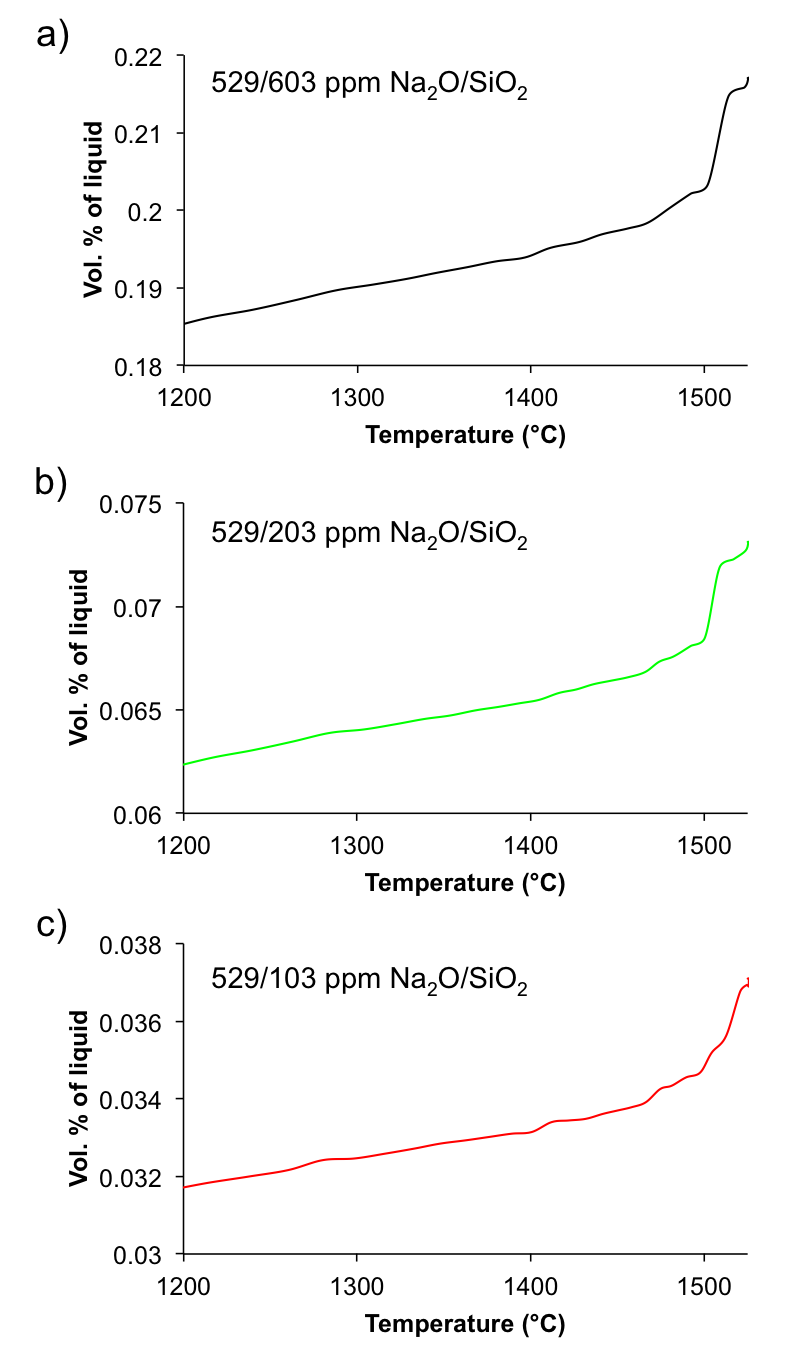
\includegraphics[scale=0.8]{Chapter-4/Figures/Figure1.png}
	\caption{Increase in concentration of liquid phase as a function of temperature for MgO-free powder samples with 529 ppm Na$_{2}$O and different SiO$_{2}$ concentrations.}
	\label{Ch4-figure:Figure1}
\end{figure}
%%%

\newpage
%%%
\begin{figure}[H]
	\centering
	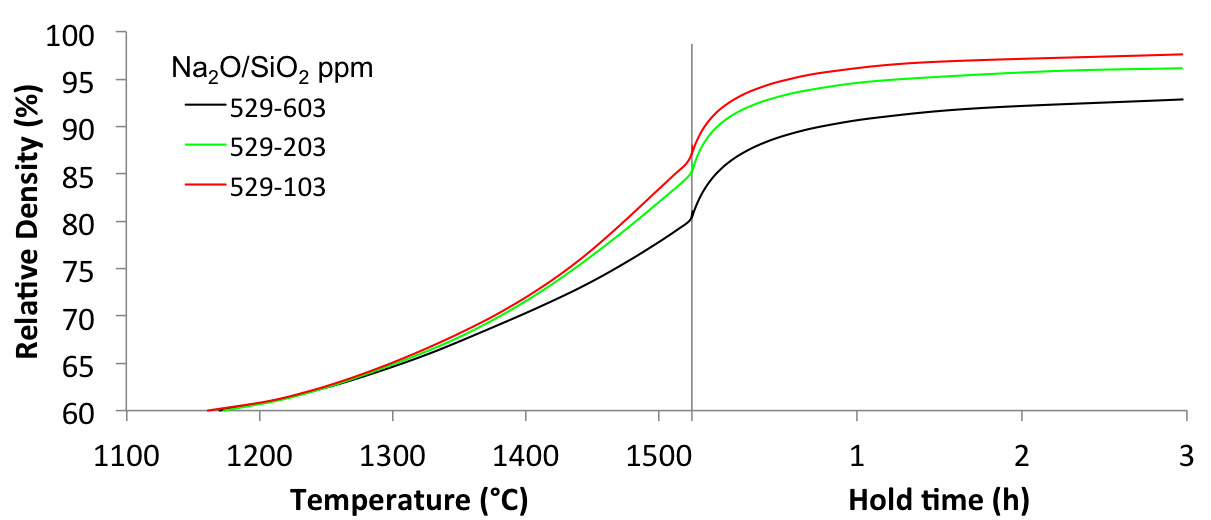
\includegraphics[width=\textwidth]{Chapter-4/Figures/Figure2.png}
	\caption{Relative density as a function of temperature and hold time determined from dilatometry for MgO-free powder samples with 529 ppm Na$_{2}$O and different SiO$_{2}$ concentrations.}
	\label{Ch4-figure:Figure2}
\end{figure}
%%%

\newpage
%%%
\begin{figure}[H]
	\centering
	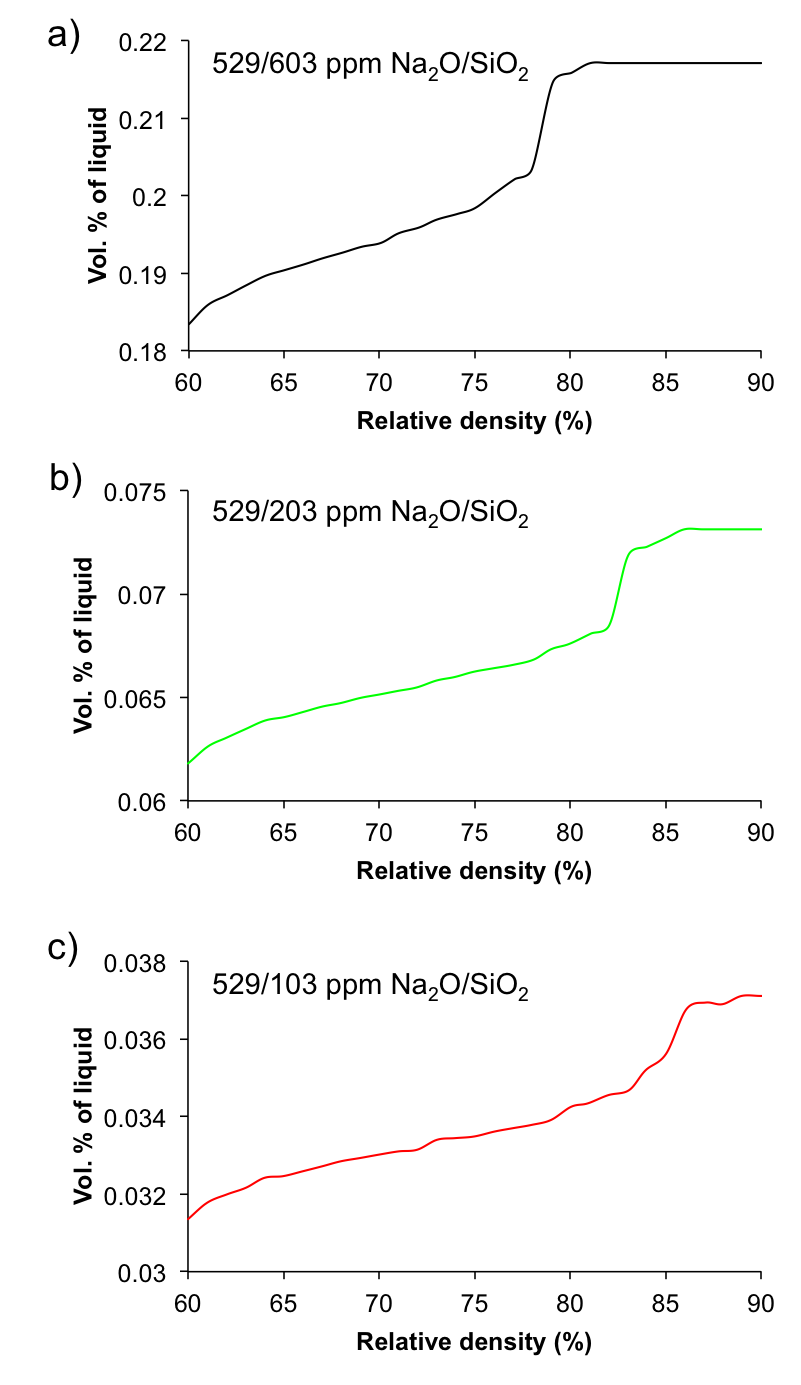
\includegraphics[scale=0.8]{Chapter-4/Figures/Figure3.png}
	\caption{Liquid phase concentration as a function of relative density for MgO-free powder samples with 529 ppm Na$_{2}$O and different SiO$_{2}$ concentrations.}
	\label{Ch4-figure:Figure3}
\end{figure}
%%%

\newpage
%%%
\begin{figure}[H]
	\centering
	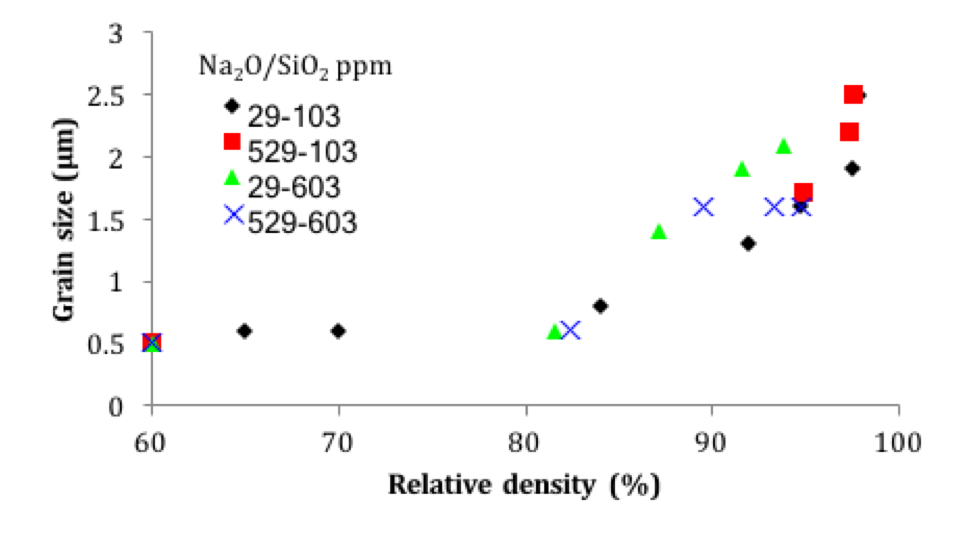
\includegraphics[width=\textwidth]{Chapter-4/Figures/Figure4.png}
	\caption{Grain size - density trajectories as a function of Na$_{2}$O and SiO$_{2}$ concentration for MgO-free alumina.}
	\label{Ch4-figure:Figure4}
\end{figure}
%%%

\newpage
%%%
\begin{figure}[H]
	\centering
	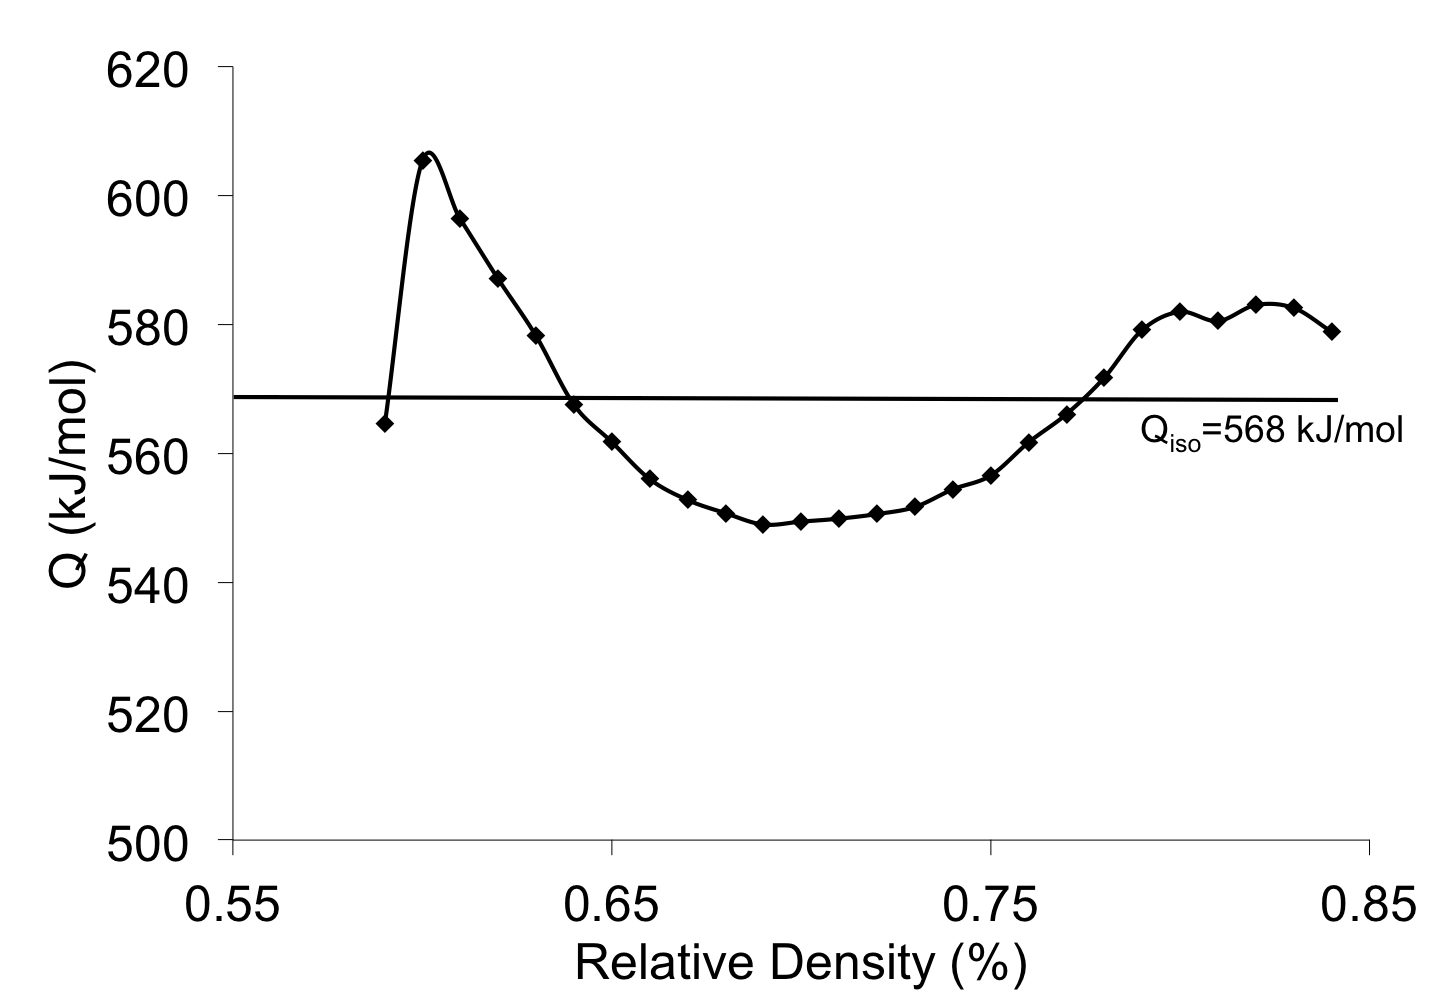
\includegraphics[width=\textwidth]{Chapter-4/Figures/Figure5.png}
	\caption{Contributions to the equilibrium film thickness as a function of film thickness for MgO-free powder samples with 529/603 ppm Na$_{2}$O/SiO$_{2}$ at a relative density of 93\%.}
	\label{Ch4-figure:Figure5}
\end{figure}
%%%

\newpage
%%%
\begin{figure}[H]
	\centering
	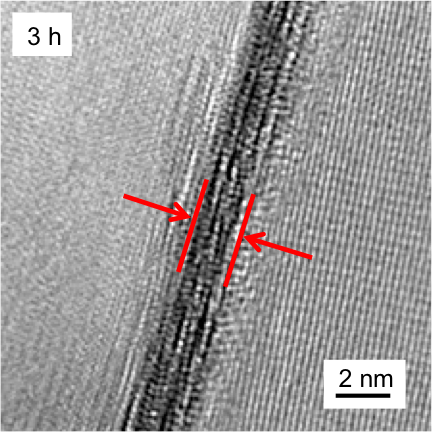
\includegraphics[width=\textwidth]{Chapter-4/Figures/Figure6.png}
	\caption{Calculated equilibrium film thickness for MgO-free powder samples at different chemistries as a function of relative density.}
	\label{Ch4-figure:Figure6}
\end{figure}
%%%

\newpage
%%%
\begin{figure}[H]
	\centering
	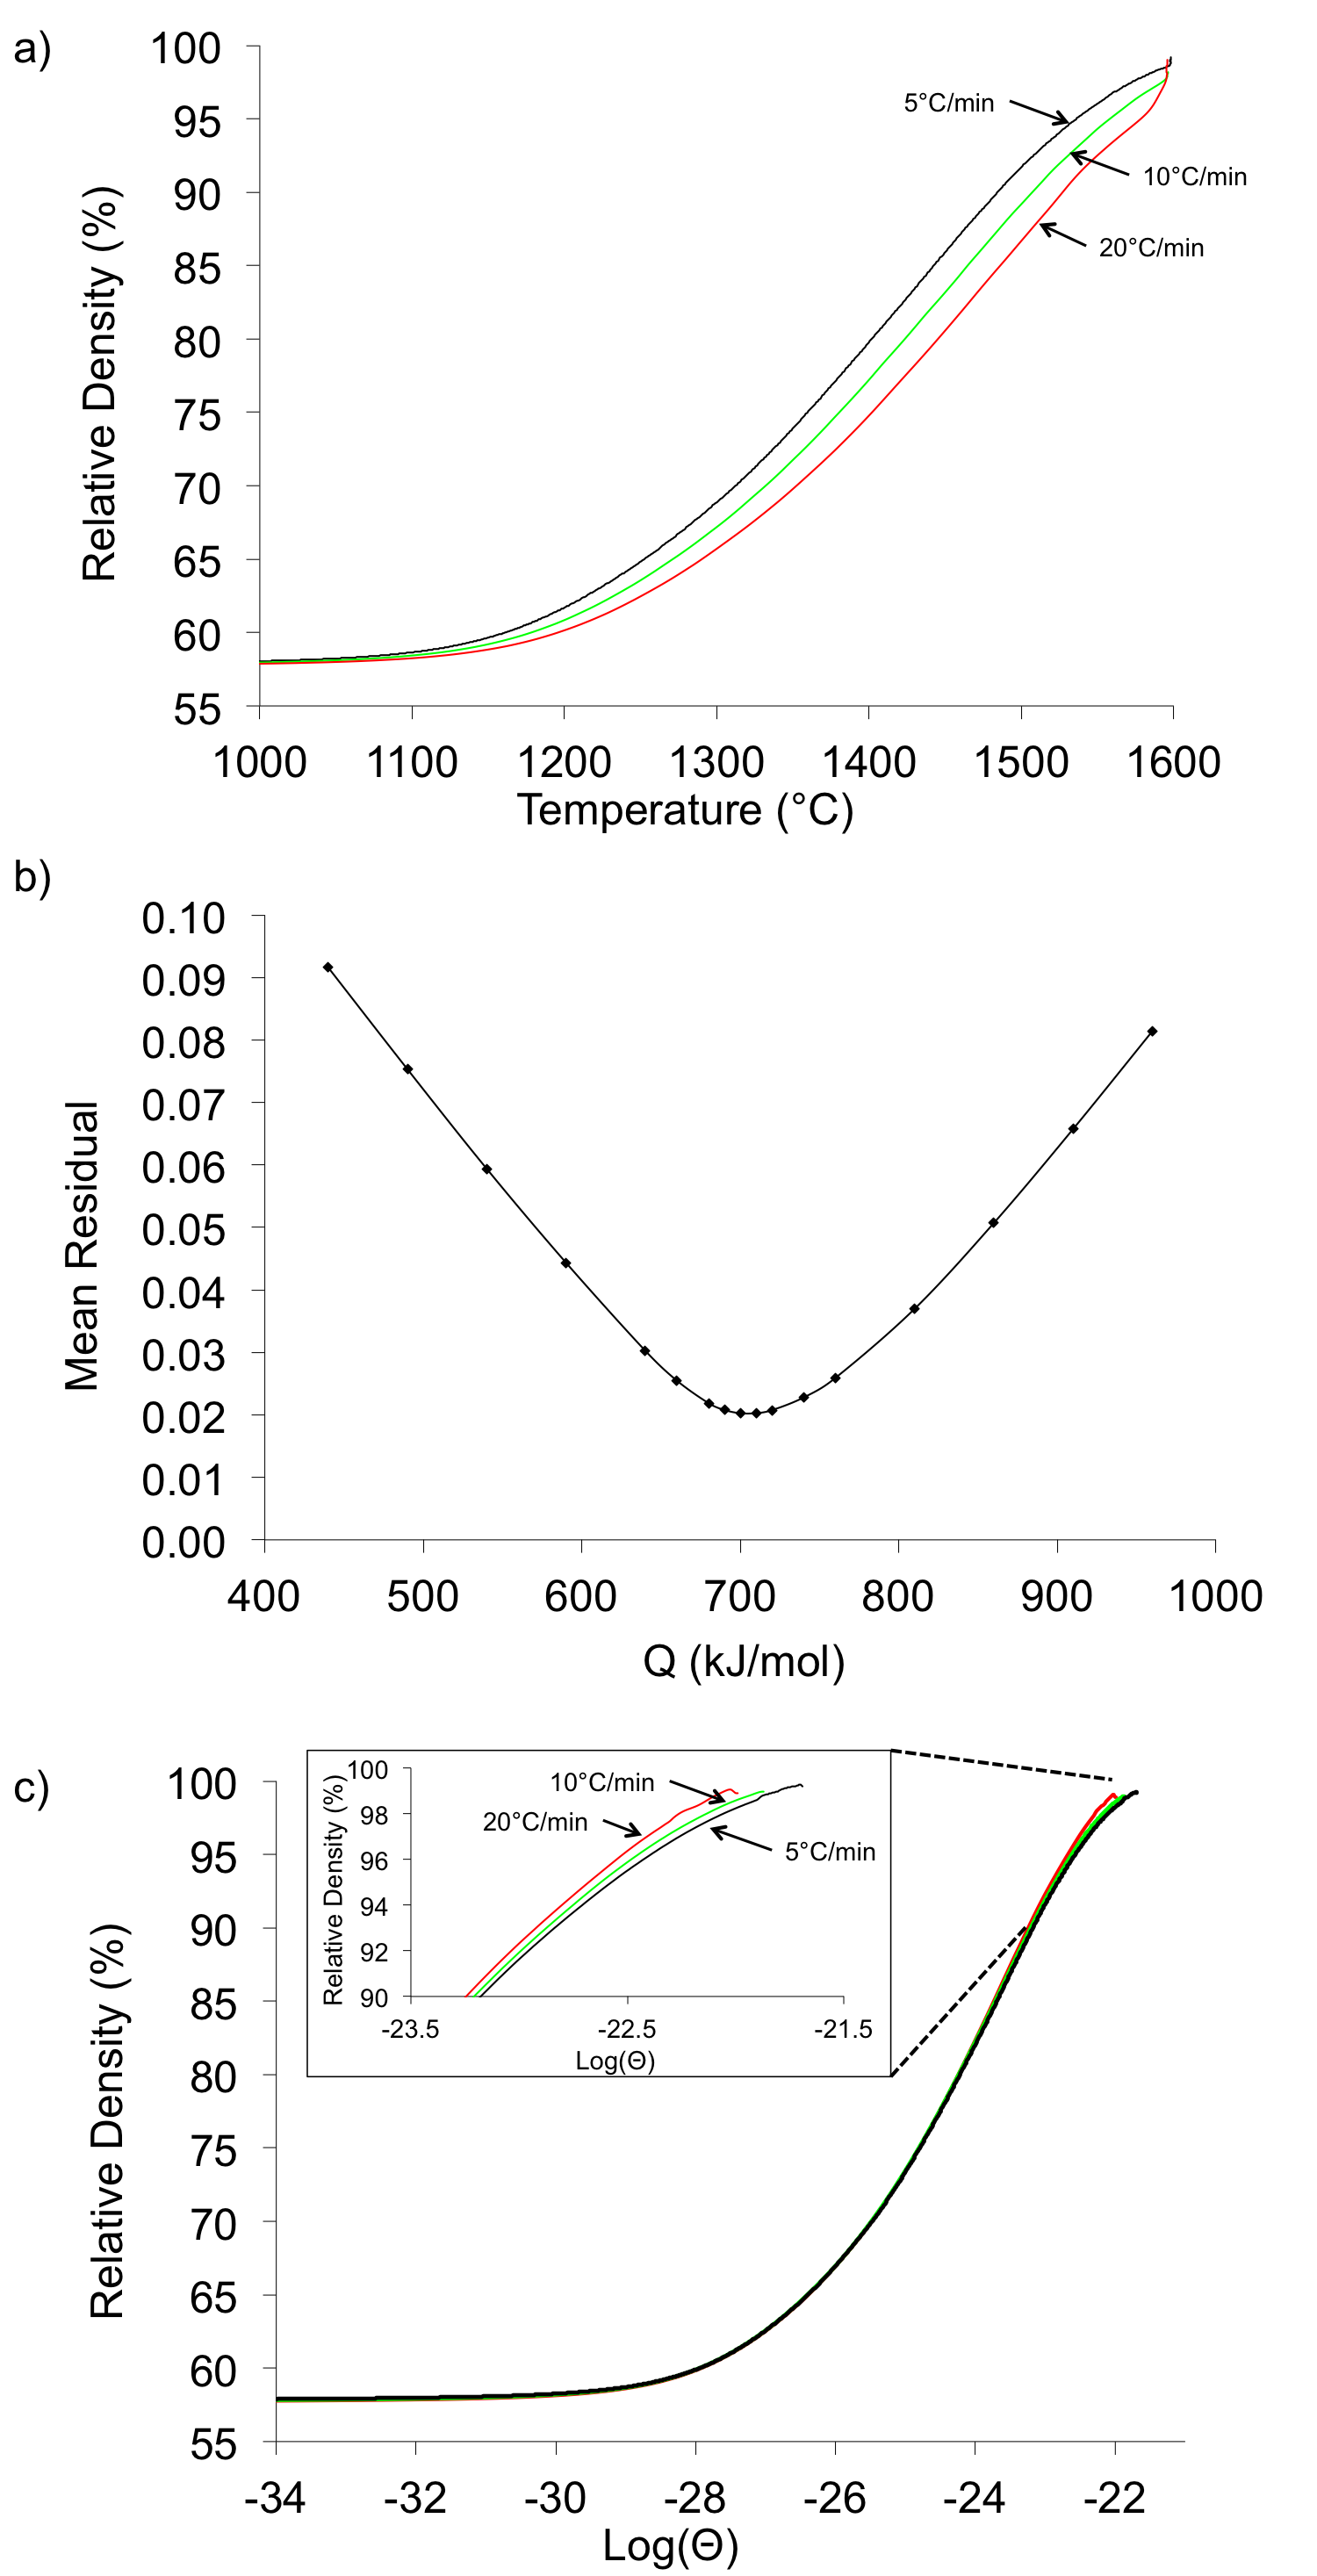
\includegraphics[width=\textwidth]{Chapter-4/Figures/Figure7.png}
	\caption{Calculated grain boundary thicknesses as a function of relative density for MgO-free powder samples. The trajectories labeled with 529/603 ppm Na$_{2}$O/SiO$_{2}$, 529/203 ppm Na$_{2}$O/SiO$_{2}$, and 529 ppm Na$_{2}$O/SiO$_{2}$ were calculated based on the liquid phase concentration and sintering stage. The equilibrium film thickness was calculated based on Clarke's model. The calculated grain boundary thicknesses are compared to measured grain boundary thicknesses (data points a: 1000/1000 ppm Na$_{2}$O/SiO$_{2}$, b) 529/603 ppm Na$_{2}$O/SiO$_{2}$, c) 529/203 ppm Na$_{2}$O/SiO$_{2}$ after heating at 1525$^{\circ}$C for 3 h).}
	\label{Ch4-figure:Figure7}
\end{figure}
%%%

\newpage
%%%
\begin{figure}[H]
	\centering
	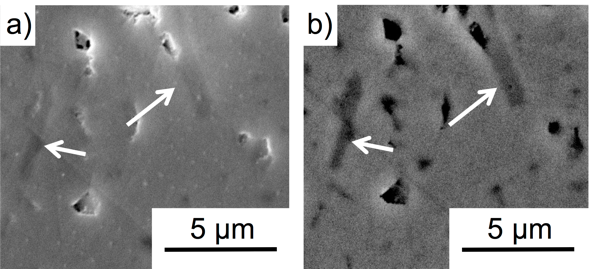
\includegraphics[width=\textwidth]{Chapter-4/Figures/Figure8.png}
	\caption{TEM images of MgO-free powder samples with a) 529/203 ppm Na$_{2}$/SiO$_{2}$, b) 529/603 ppm Na$_{2}$/SiO$_{2}$, c) 1000/1000 ppm Na$_{2}$/SiO$_{2}$, and d) 29/103 ppm Na$_{2}$/SiO$_{2}$ after sintering at 1525$^{\circ}$C for 3 h.}
	\label{Ch4-figure:Figure8}
\end{figure}
%%%

\newpage
%%%
\begin{figure}[H]
	\centering
	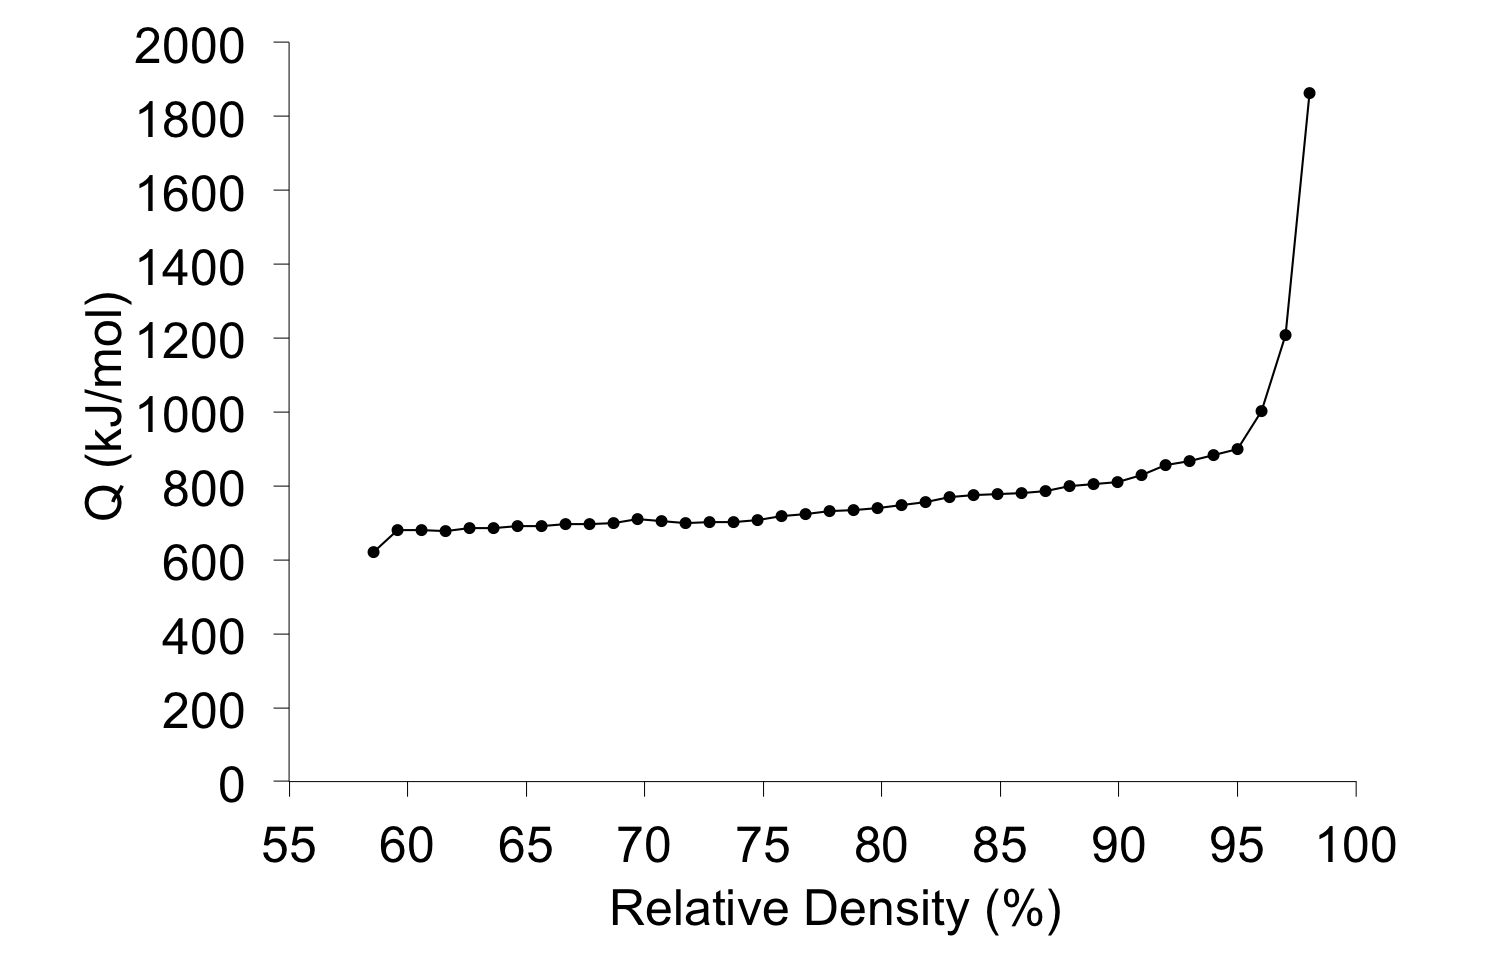
\includegraphics{Chapter-4/Figures/Figure9.png}
	\caption{TEM image of a MgO-free powder sample with 29/603 ppm Na$_{2}$O/SiO$_{2}$.}
	\label{Ch4-figure:Figure9}
\end{figure}
%%%

\newpage
%%%
\begin{figure}[H]
	\centering
	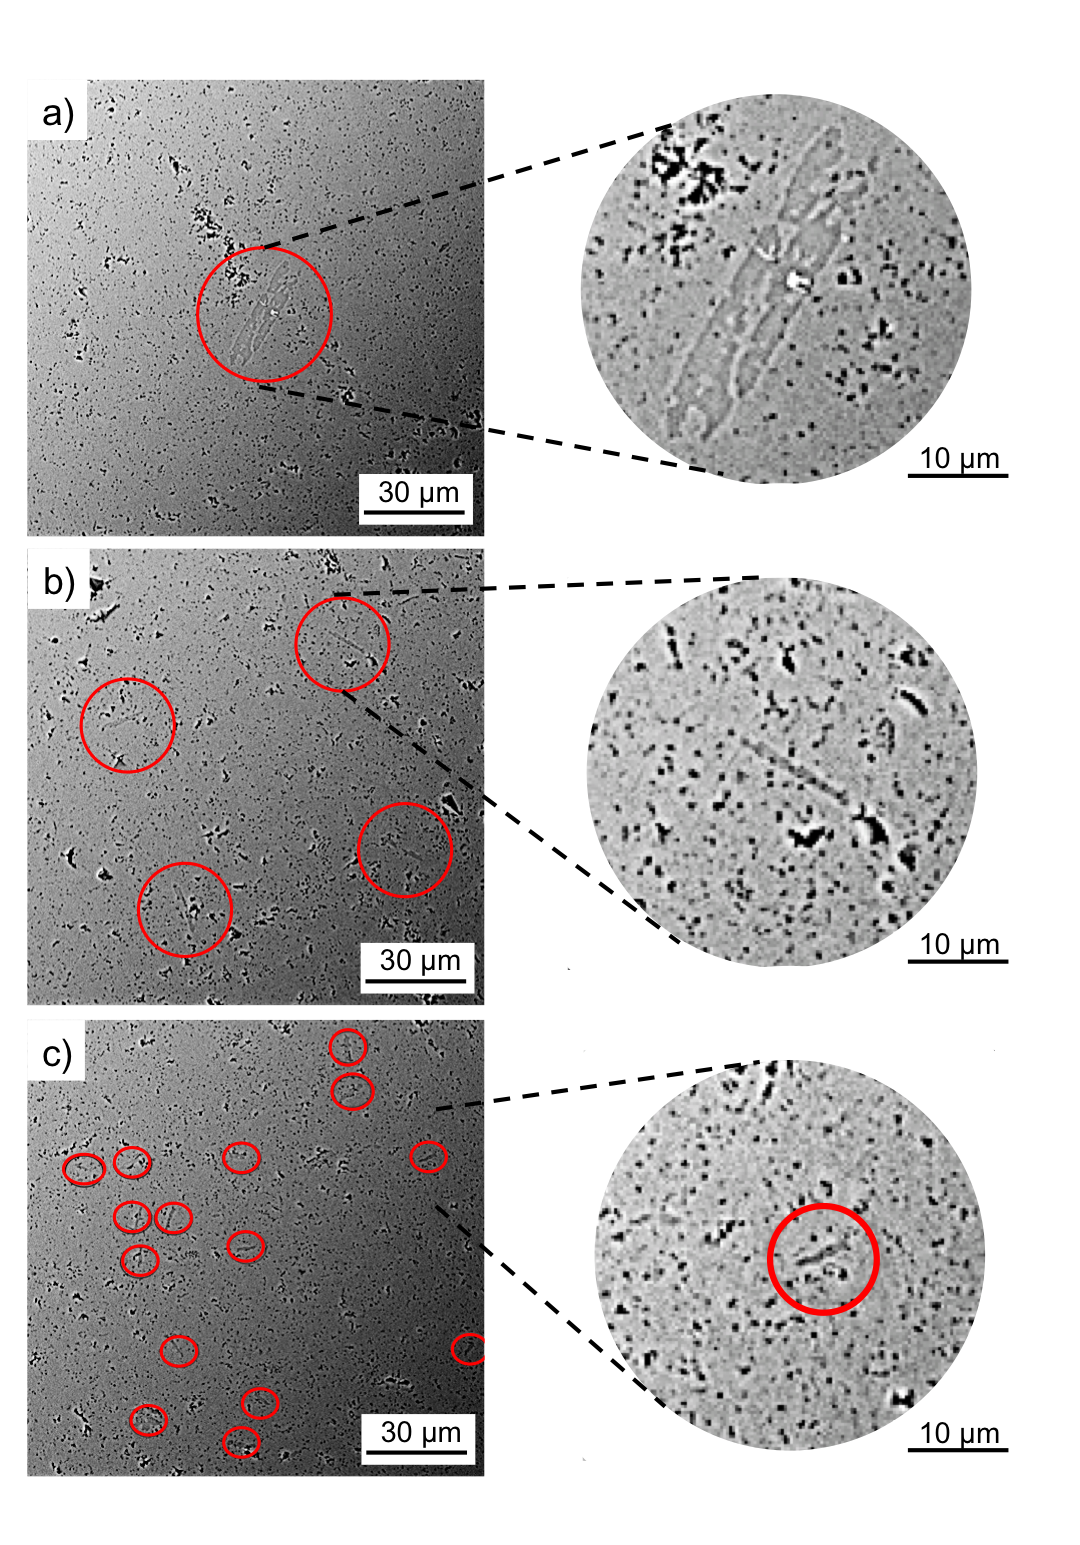
\includegraphics{Chapter-4/Figures/Figure10.png}
	\caption{TEM images of MgO-doped (380 ppm) powder samples with a) 60/82 ppm Na$_{2}$O/SiO$_{2}$, b) 60/582 ppm Na$_{2}$O/SiO$_{2}$, and c) 560/582 ppm Na$_{2}$O/SiO$_{2}$. After heating at 1525$^{\circ}$C for 3 h.}
	\label{Ch4-figure:Figure10}
\end{figure}
%%%
